\documentclass[12pt]{exam}

% ---------------------------------------------------
% Page Layout
% ---------------------------------------------------
\usepackage{geometry}   % Flexible page dimensions
\geometry{margin=1in, centering}

% ---------------------------------------------------
% Encoding and Fonts
% ---------------------------------------------------
\usepackage[utf8]{inputenc}   % Input encoding
\usepackage[T1]{fontenc}      % Output font encoding
\usepackage{lmodern}          % Latin Modern fonts (improves output)

% ---------------------------------------------------
% Tables and Columns
% ---------------------------------------------------
\usepackage{multicol}   % Multiple column environments
\usepackage{multirow}   % Multi-row cells in tables
\usepackage{booktabs}   % Better looking tables

% ---------------------------------------------------
% Graphics and Figures
% ---------------------------------------------------
\usepackage{graphicx}   % Include graphics
\usepackage{caption}    % Customization of captions

% ---------------------------------------------------
% Text Styling
% ---------------------------------------------------
\usepackage{color}      % Color support
\usepackage{soul}       % Highlighting, underlining, strikethrough, etc.

% ---------------------------------------------------
% Headers, Footers, and Symbols
% ---------------------------------------------------
\usepackage{lastpage}   % Reference last page in document
\usepackage{bbding}     % Special symbols (checkmarks, etc.)
\usepackage{pmboxdraw}  % Box drawing characters
\usepackage{fontawesome} % Allows customization of icons 

% ---------------------------------------------------
% Section Formatting
% ---------------------------------------------------
\usepackage{titlesec}   % Customize section titles

% ---------------------------------------------------
% Hyperlinks and URLs
% ---------------------------------------------------
\usepackage{url}        % Simple URL typesetting
\usepackage{hyperref}   % Clickable hyperlinks


\titleformat{\section}
  {\normalfont\large\bfseries\sffamily}{\thesection}{1em}{}

\titleformat{\subsection}
  {\normalfont\normalsize\bfseries\sffamily}{\thesection}{1em}{}
  
\hypersetup{
    colorlinks=true,
    linkcolor=blue,
    filecolor=magenta,      
    urlcolor=blue,
    citecolor=blue,
}

% ---------------------------------------------------
% Multiple Choice Options 
% ---------------------------------------------------
\CorrectChoiceEmphasis{\color{red}\bfseries\itshape}

% ---------------------------------------------------
% Defines Header & Footer Content
% ---------------------------------------------------
% This is the name of the course (left header)
\newcommand{\class}{\fontfamily{lmss} \textbf{EC 390}} 
% This is the name of the assignment (center header)
\newcommand{\examnum}{\fontfamily{lmss} \textbf{PS 02}} 
% This is the due date (right header)
\newcommand{\examdate}{\fontfamily{lmss} \textbf{October 22 at 11:59am}} 

% ---------------------------------------------------
% Points Options
% ---------------------------------------------------
\addpoints              % Allows to add points up to include table at end of document
\bracketedpoints        % Puts points per question inside brackets instead of parenthesis 
%\printanswers
% ---------------------------------------------------
% Header & Footer Options
% ---------------------------------------------------
\pagestyle{headandfoot}         % Fancy equivalent for exam documentclass
\firstpageheadrule              % Horizontal bar in first page
\runningheadrule                % Horizontal bar in rest of pages

% 1st page header content
\firstpageheader{\class}{}{\fontfamily{lmss} Due \examdate} 
% Rest of pages header content
\runningheader{\class}{\examnum}{\fontfamily{lmss} Due \examdate} 

% 1st page footer content
\firstpagefooter{\fontfamily{lmss} Points earned: \makebox[1in]{\hrulefill} / \pointsonpage{\thepage} points}{}{\thepage\ of \numpages} 
% Rest of pages footer content
\runningfooter{\fontfamily{lmss} Points earned: \makebox[1in]{\hrulefill} / \pointsonpage{\thepage} points}{}{\thepage\ of \numpages} 

% ---------------------------------------------------
% Section Formatting & Options
% ---------------------------------------------------
\titleformat{\section}
  {\normalfont\large\bfseries\sffamily}{\thesection}{1em}{}

\titleformat{\subsection}
  {\normalfont\normalsize\bfseries\sffamily}{\thesection}{1em}{}

% ---------------------------------------------------
% Body Begins
% ---------------------------------------------------
\begin{document}

\fontfamily{lmss}\selectfont

\begin{center}
    \textbf{{\LARGE EC 390 Problem Set 02}} \\
    \smallskip 
\end{center}

% ---------------------------------------------------
% Instructions
% ---------------------------------------------------
\noindent \textbf{Instructions:} 
Answers must be submitted online through the designated Canvas assignment in a \textbf{PDF file}.
Any other file type is not allowed. 
This Problem Set is due on \examdate.
Please write as legible and clearly as possible. 
You will not be given full credit if your answers cannot be easily understood. 

% ---------------------------------------------------
% Questions Begins
% ---------------------------------------------------
\section*{Questions}

\begin{questions}
    
\question[10] 
Take the following Average Total Cost Curves below.
Firm 1 is an \textbf{incumbent firm} and is represented by the orange ATC curve.
Firm 2 is an \textbf{entering firm} and is represented by the blue ATC curve. 
They both produce at their shown quantities $Q_{1}$ and $Q_{2}$ respectively.
The y-axis is the per unit cost and the x-axis represents quantity of goods produced. 
Explain how this graph demonstrates the \textbf{firm incumbency advantage} discussed in the multiple equilibria lecture.
Explain (Be brief in your explanation).

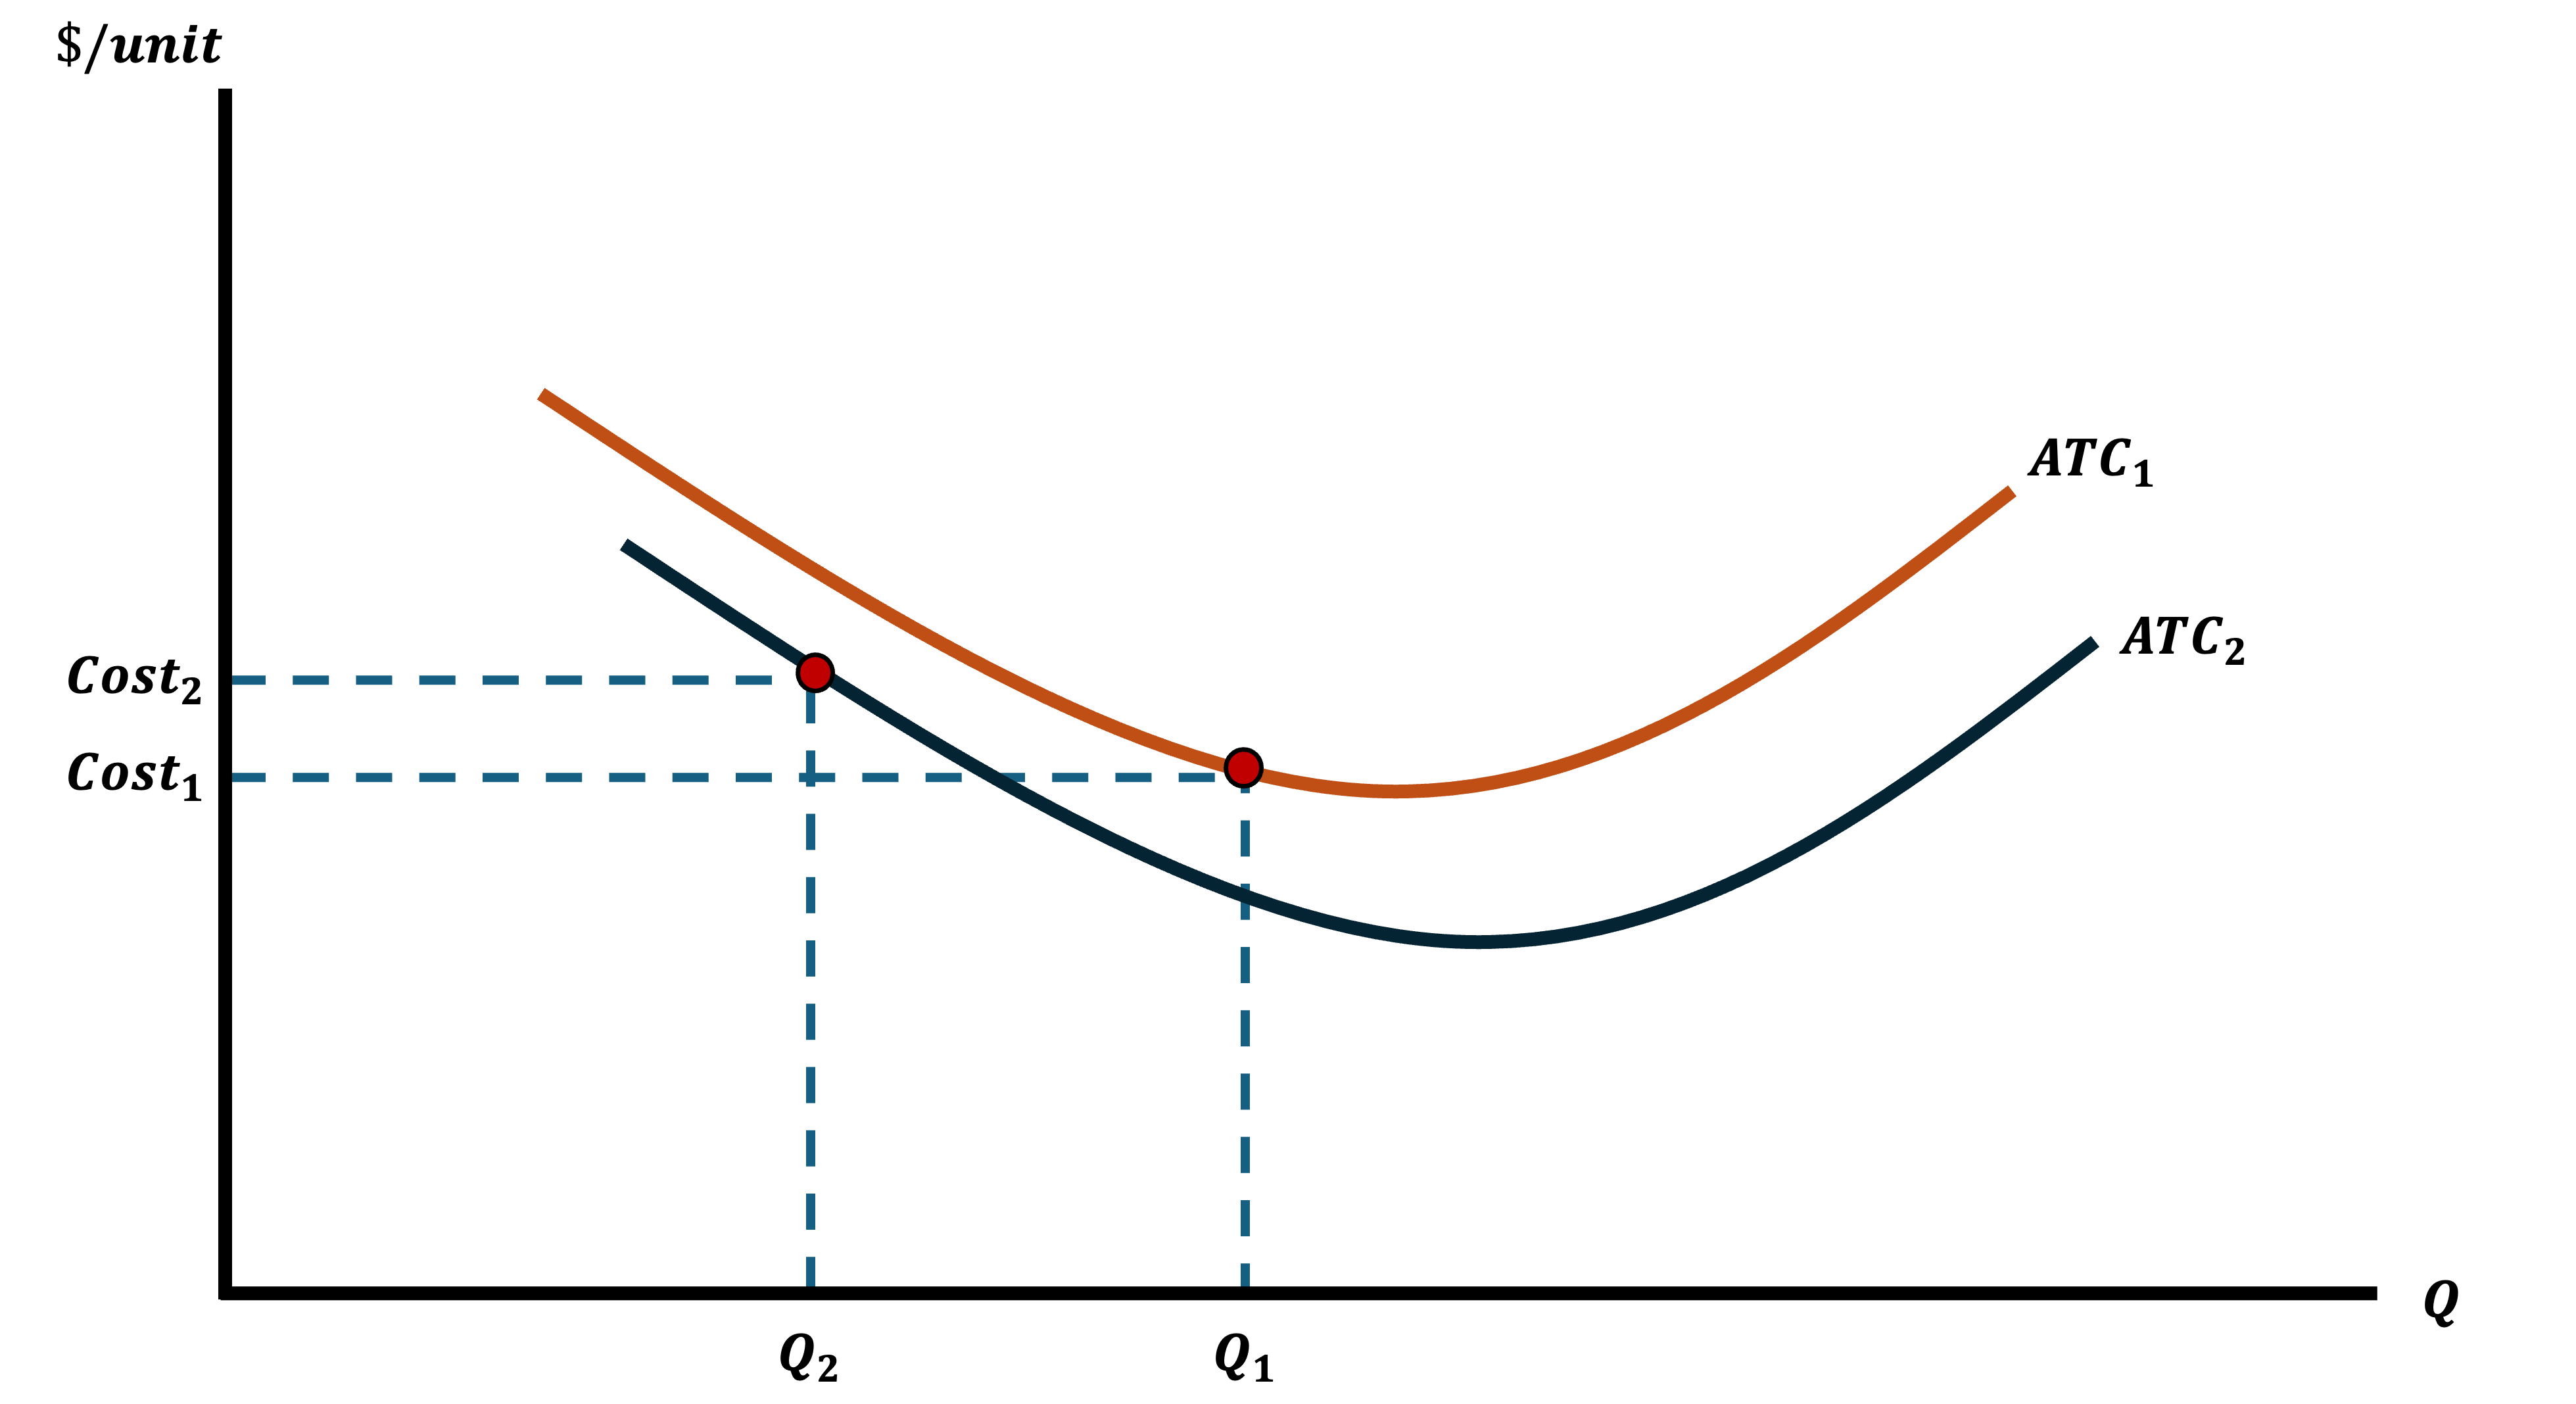
\includegraphics[scale=0.3]{images/atc-curve.png}
\vspace*{\stretch{0.5}}

\question[5]
Consider the Solow model discussed in class.
In this country, \textbf{women's labor force participation} increases which, in turn, reduces fertility rates in the country. 
At the same time, since there are fewer dependents, households \textbf{can save more}. 
Show graphically what happens to \textbf{capital per worker $(k)$} and \textbf{output per worker $(y)$}.
\vspace*{\stretch{1.5}}

\newpage 

\question[2]
When one agent's actions provide an \textbf{incentive} for other agents to take similar actions, we say that there are \fillin[complementarities][4cm] between these actions
\vspace*{\stretch{0.5}}

\question
Consider the following S-curve diagram:
\begin{center}
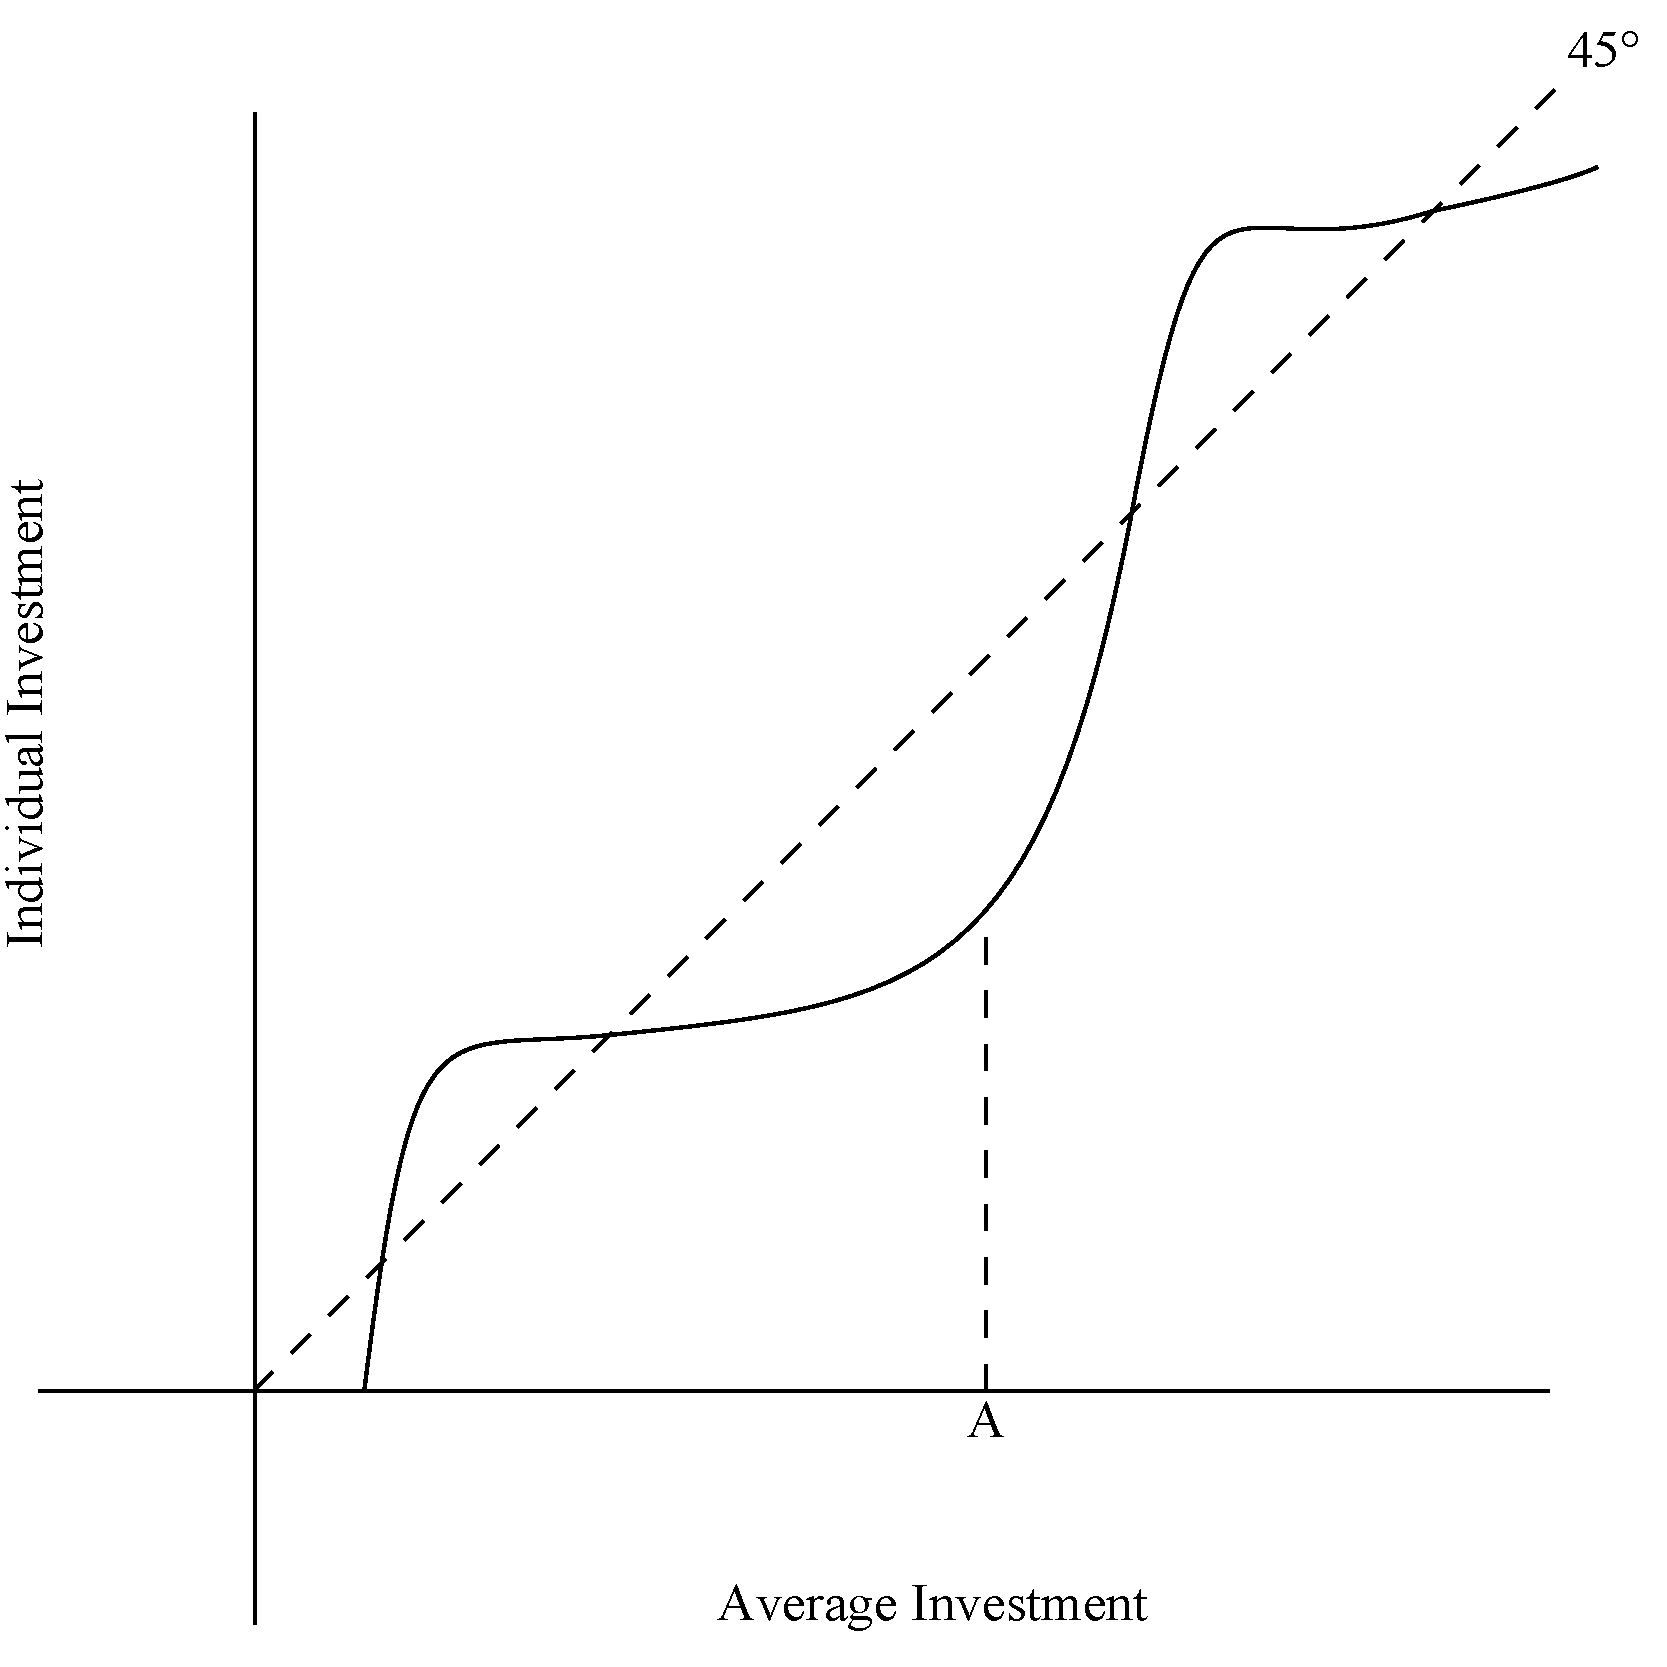
\includegraphics[scale=0.3]{images/scurve.pdf}
\vspace*{\stretch{1}}
\end{center}

\begin{parts}
  \part[2] 
  Label the equilibrium points on the graph (Make sure they are identifiable and named)
  \part[3] 
  Classify each equlibrium as \textbf{stable or unstable}
  \vspace*{\stretch{2}}
  \part[5] 
  Suppose that average investment is currently at point A. 
  Where will average investment end up?
  \textbf{Show the dynamics on the graph by drawing arrows}
  \vspace*{\stretch{1}}
\end{parts}

\newpage 

\question
Consider the following Lorenz Curve

\begin{center}
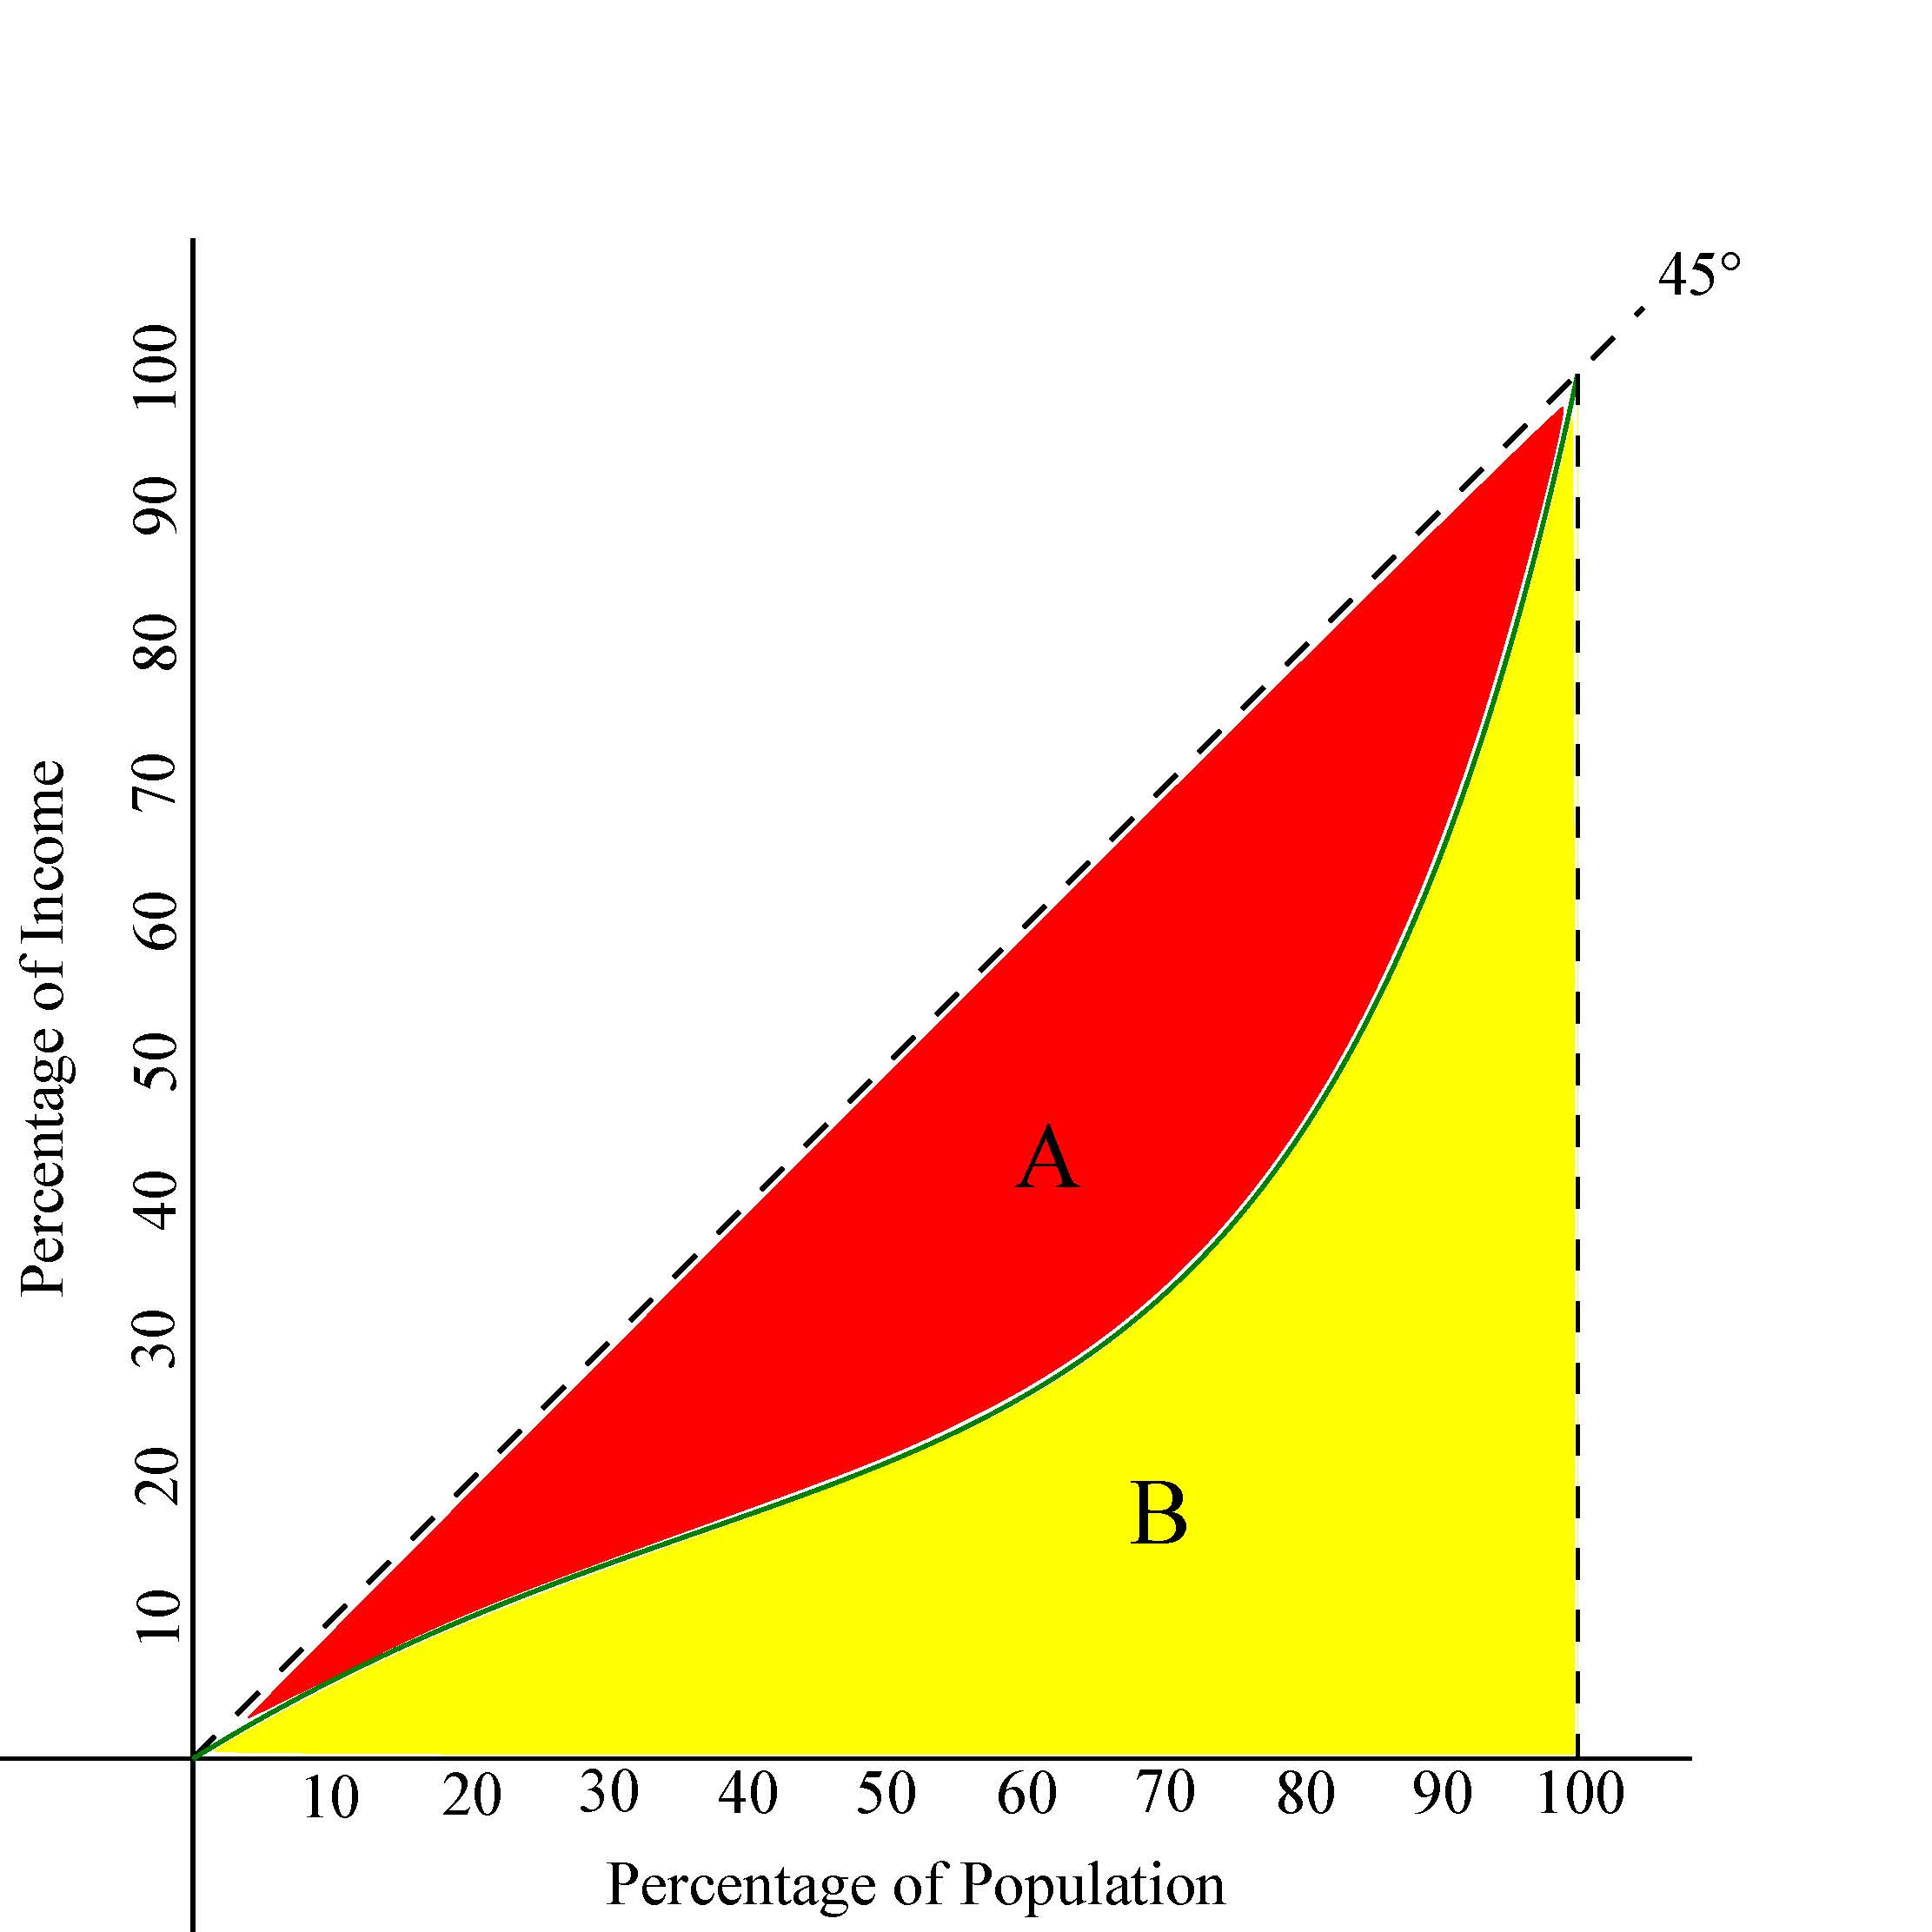
\includegraphics[scale=0.25]{images/lorenz.jpg}
\end{center}

\begin{parts}
  \part[2] 
  Describe how the \textbf{Lorenz Curve} would change if the society had \textbf{perfect income equality}
  \vspace*{\stretch{1}}
  \part[2] 
  Describe how the \textbf{Lorenz Curve} would change if the society had \textbf{perfect income inequality}
  \vspace*{\stretch{1}}
  \part[4] 
  If the we have the area of $A = 0.15$ and the area of $B = 0.35$, what is the \textbf{Gini Coefficient} for this society?
  \textbf{Show your work}
  \vspace*{\stretch{1}}
\end{parts}

\newpage 

\question 
Consider the O-Ring model.
It predicts that there will be a strong tendency for the most productive workers to work together. 
Let there be 6 workers and 2 firms, where each firm hires 3 workers total.
There are 3 high-skill $q_{H}$ workers and 3 low-skill $q_{L}$ workers, such that $q_{H} > q_{L} > 0$.
Workers can be assigned in either \textbf{sorted groups} or \textbf{mixed groups}:
\begin{itemize}
  \item \textbf{Mixed Assignment:} Firm 1 hires $(q_{H},q_{H},q_{L})$ and Firm 2 hires $(q_{H},q_{L},q_{L})$
  \item \textbf{Sorted Assignment:} Firm 1 hires $(q_{H},q_{H},q_{H})$ and Firm 2 hires $(q_{L},q_{L},q_{L})$
\end{itemize}

\begin{parts}
  \part[5] 
  Compute the total output under each \textbf{type of assignment}
  \vspace*{\stretch{1}}
  \part[10] 
  Show \textbf{algebraically} that the sorted assignment yields striclty higher total output whenever $q_{H} > q_{L}$
  \vspace*{\stretch{2}}
\end{parts}

\end{questions}

\end{document}